%%%%%%%%%%%%%%%%%%%%%%% file template.tex %%%%%%%%%%%%%%%%%%%%%%%%%
%
% This is a template file for RO 
%
% Copy it to a new file with a new name and use it as the basis
% for your article
%
%%%%%%%%%%%%%%%%%%%%%%%%   EDP Sciences  %%%%%%%%%%%%%%%%%%%%%%%%%%
%
\documentclass{ro}
%
%%%%%%%%%%%%%--PREAMBLE--%%%%%%%%%%%%%%%%%%
%%-----------------------------
%

\usepackage{graphicx}
\usepackage{algorithm}
\usepackage{algorithmic}
%\usepackage{multicol}
%\usepackage{subfigure}
%\usepackage{cite}
%\usepackage[authoryear]{natbib}
\usepackage{mathtools}
\usepackage{url}
\usepackage{xcolor}
\usepackage{enumerate}
\usepackage{color}
\usepackage{ctable}


\DeclarePairedDelimiter{\ceil}{\lceil}{\rceil}
\DeclarePairedDelimiter{\floor}{\lfloor}{\rfloor}
\newcommand\numberthis{\addtocounter{equation}{1}\tag{\theequation}}

\usepackage{lineno}
%\linenumbers


%
% \usepackage{mathptmx}      % use Times fonts if available on your TeX system
%
% insert here the call for the packages your document requires
%\usepackage{latexsym}
% etc.
%
% please place your own definitions here and don't use \def but
% \newcommand{}{}
%
% Insert the name of "your journal" with
%

%\allowdisplaybreaks

%         your macros
%         ...........
%%-------------------------%%----
%%%%%%%%%%%%%%%--BODY--%%%%%%%%%%%%%%%%%%
\allowdisplaybreaks
\begin{document}
%%-----------------------------
%%      the top matter
%%-----------------------------
\title{Reactive GRASP for the Prize-collecting Covering Tour Problem}% At most 5 thanks
%
\author{Glaubos Cl\'imaco*}\address{Universidade Federal do Maranhão, Av. dos Portugueses, 1966 - Vila Bacanga, Sao Lu\'is, Brasil.}\thanks{Corresponding author: francisco.glaubos@ufma.br}

\author{Isabel Rosseti}\address{ Universidade Federal Fluminense, Instituto de Computa\c{c}\~ao. Rua Passo da P\'atria 156 S\~ao Domingos 24210-240 - Niter\'oi, RJ - Brasil}

\author{Rog\'erio da Silva}\address{Institute of Education, Science and Technology of Piau\'i.R. Alvaro Mendes, 94 - Centro (Sul), Teresina - Brasil}

\author{Marcos Guerine}\address{Federal Institute of Education, Science and Technology of Rio de Janeiro.  Rua Jos\'e Breves, 550, Centro, Pinheiral, RJ, Brazil}


%
\date{...}
%
\begin{abstract} 

This paper presents a greedy randomized adaptive search procedure (GRASP) for the prize-collecting covering tour problem, which is the problem
of finding a route for traveling teams that provide services to communities geographically distant from large urban locations. We devised a novel hybrid heuristic by combining a reactive extension of the GRASP with Random Variable Neighborhood Search (VND) meta-heuristic for the purpose of solving the PCCTP. Computational experiments were conducted on a PCCTP benchmark from the literature, and the results demonstrate our approach provides a significant improvement in solving PCCTP and comparable with the state-of-the-art, mainly regarding the computational processing time.

 \end{abstract}
%

%we evaluate our methods with instances of the literature with very satisfactory results.

\subjclass{???, ???}
%
\keywords{prize-collecting covering tour problem,  hybrid heuristic, GRASP, VND}
%
\maketitle
%%-----------------------------
%%      your text
%%-----------------------------


\section{Introduction}
\label{sec:intro}
The provision of social, medical or, legal assistance to communities geographically distributed and distant from large urban centers has been a concern of the various public, philanthropic or private entities. Deploying fixed units in these locations involves significant investments, and there is still a shortage of professionals with interest in being in those regions.


One of the most appropriate	solutions is to attend to people who live in places far from the service centers is the use of traveling teams. As an example, the Brazilian Courts of Justice (TJ) have a project called Itinerant Justice, in which an adapted bus with a full forum structure is used to perform most of the legal services. This bus periodically arrives at cities far from the TJ units, thus covering a large number of citizens unable to have legal assistance. 

In this context, the prize-collecting covering tour problem (PCCTP) arises. The objective of this problem is to find a minimum cost tour that passes through some mandatory cities ($T$) and, sometimes, others that are not mandatory ($R$). Each city has an associated prize, which represents the number of people served if the tour passes through it. Some cities may be inaccessible ($W$), and their inhabitants must travel to the closest city to receive assistance. Besides, the tour must guarantee a minimum attendance of people, so that the trip of a TJ bus is worthwhile.


The PCCTP is an NP-hard problem as it generalizes the  NP-hard covering tour problem (CTP) \cite{gendreau1997covering}. Since it was first introduced by Gendreau \textit{et al.} \cite{gendreau1997covering}, several generalizations of the CTP have been proposed. Some of these variants refer to multi vehicles that must: collectively cover the cities of $W$ \cite{hachicha2000heuristics}; minimize the sum of arrival times at visited locations, while the total duration of each tour does not exceed a preset time limit \cite{flores2017multi}; cover cities of $W$ more than once \cite{pham2017solving}; and,  handle a probabilistic coverage while maximizes the expected customer demand covered \cite{karaouglan2018multi}. Other generalizations are three bi-objective  versions that despite the traditional CTP objective: include the minimization of the cover \cite{jozefowiez2007bi};  maximize the number of covered cities $W$ \cite{ebrahimi2012maximal}; and, incorporate the minimization of expected uncovered stochastic demand \cite{tricoire2012bi}.

All the aforementioned generalizations  emerged from real-world needs that have not been considered by the classic CTP. In this work, we address the prize-collecting covering tour problem (PCCTP), in which every city $v \in V$ is associated with a prize $p_v$, and the tour must guarantee a preset minimum prize collection. This type of generalization, with prizes to be collected at the vertices, is common in the literature and has been widely addressed in other problems such as the traveling salesman problem \cite{berube2009branch}, vehicle routing problem \cite{trachanatzi2020firefly}, and Steiner tree problem \cite{canuto2001local}.


This problem is relatively new in the literature and there are two mathematical formulations describing it. The first one was proposed by Lyra \cite{lyra2004problema} along with the problem and makes use of constraints based on flow to eliminate sub-routes in the solution. The second one was proposed by  Silva \cite{silva2009problema}, and it is based on multi-flow constraints to
handle with sub-routes in the solution.


Since PCCTP is an NP-Hard problem, it is impracticable to solve large instances ($|N|$ greater than 100) using only exact methods \cite{lyra2004problema}. Therefore, heuristic approaches are required to deal with such instances. Lyra \cite{lyra2004problema} proposed a heuristic based on GRASP combined with a variation of the VNS (Variable neighborhood Search) metaheuristic \cite{mladenovic97}. Its heuristic approach also includes a path-relinking technique as an improving solutions component.

In the following,  Silva \cite{silva2009problema} proposed new six heuristic methods, in which five of them are based on the ILS (Iterated Local Search)  meta-heuristic \cite{lourencco2003iterated}, and one is an evolutionary heuristic. Silva \cite{silva2009problema} conducted experiments on test-problems proposed in his work and the ILS-RDM-CI was the one with the best overall performance. 

The ILS-RDM-CI starts by generating an initial random solution through the cheapest Insertion (CI)  heuristic. Then, at each iteration, a disturbance routine is performed followed by a Random Descent Method (RDM) procedure. The RDM applies a random movement over the best current solution ($S$) to generate a new neighbor solution $N(S)$. If this neighbor is better than the $S$, $N(S)$ becomes the new best current solution. Otherwise, another neighbor is generated. The RDM method stops when a maximum number of iterations without improvement is reached, and the whole ILS-RDM-IC heuristic stops when a maximum number of disturbances is reached.


In this paper, we propose a hybrid heuristic derived from the reactive GRASP (Greedy Randomized Adaptive Search Procedure) metaheuristic \cite{grasp03}  for solving the prize-collecting covering tour problem. The GRASP metaheuristic is performed, iteratively, in two main phases: constructive and local search. The first phase is based on a GENIUS heuristic \cite{genius} adapted for the PCCTP, while in the second phase, several moves are designed and combined in a VND (Random Variable neighborhood Descent) structure \cite{mladenovic97}. The resulting R-GRASP heuristic is fast, and the extensive computational results show the solutions to be equal to or better than those obtained by the best existing heuristic ILS-RDM-CI. Besides, we have implemented and tested the two mathematical formulations from the literature  using a mixed-integer linear programming (MILP) solver, and compared the results with the heuristic.


% which has presented  better performance in finding optimal solutions than the Lyra's \cite{silva2009problema}. We have implemented the formualtion  formulation using an mixed integer programming solver, and compared the results with the heuristics.


The remainder of this paper is organized as follows. Section \ref{sec:prob} defines formally the PCCTP and its existing mathematical formulations. Section \ref{sec:metod} shows the proposed R-GRASP 
heuristic. Section \ref{sec:results} presents the computational results obtained by the proposed and the state-of-the-art heuristics; and in Section \ref{sec:conclusions}, some conclusions, and a few future works are drawn.



\section{Problem definition}
\label{sec:prob}
The definition of the PCCTP can be given as follows. Consider an undirected graph $G = (N,E)$, with the set of vertices $N = V \cup W $ and  $V = R \cup T$.  Let $D$ be a coverage distance, $c_e$ be a cost associated to each $e \in E $ and $p_i$  be a prize associated to each vertex  $i \in V$. Let $T$ be a subset containing the vertices that must be visited and R a subset of vertices that are optional, and therefore may or may not be visited. Finally, let  $W$ be a subset containing the vertices that must be covered by another vertex from $V$, i.e., a vertex $i \in V$ covers a vertex $j \in W$ if  $c_{ij} \leq D$. The goal of the PCCTP is to find a simple minimum cost cycle that visits all vertices in $T$, covers all vertices of $W$ and collects at least a minimum prize (\textit{PRIZE}). In Figure \ref{fig:pcctp} is depicted a solution for an example of the PCCTP, in which the value of \textit{PRIZE} was set to 100.

%\begin{figure*}
%	\caption{A Sample SciPort Document}\label{fig:sampledocument}
%	\centerline{\epsffile{E:/Inderscience/LATEX-FILES/IJMSO/F1.eps}}
%\end{figure*}

\begin{figure}[t]
	\centering
	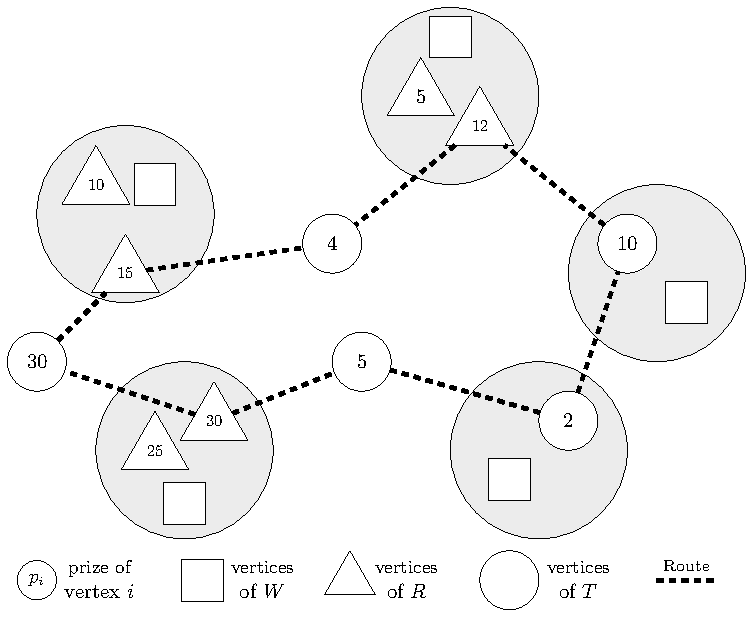
\includegraphics[width=0.7\textwidth]{pcctp-solution.pdf}
	\caption{Example of a PCCTP solution.}
	\label{fig:pcctp}
\end{figure}


A real-world application for the PCCTP can be seen in the provision of a route for the TJ's bus case, mentioned in Section \ref{sec:intro}. The vertices of $T$ would represent cities of a particular and important region  and thus are defined as mandatory visiting points, while the vertices in $R$ would represent cities in which the visits are optional. There is also a set of cities that shall be attended, but for some reason, it is impracticable and their population must be served by some neighboring cities whose distance is at most $D$ unities away, avoiding large displacement of people. These last set of cities would be represented by the vertices in $W$. To be worth the release of a bus, it is necessary that a minimum number of people be attended. Therefore, the population of each city in $T$   and $R$ is represented by the prize of each vertex, and the total \textit{PRIZE} to be collected corresponds to the minimum total number of citizens to be served. 

\subsection{Mathematical formulations}

In the literature, there are two mathematical formulations for the PCCTP. The first formulation, proposed by Lyra \cite{lyra2004problema}, uses flow variables to avoid the formation of disconnected cycles. The other formulation proposed by Silva \cite{silva2009problema}, uses multi-flow variables to avoid sub-cycles in the route.



In this section, let $G=(V,A)$ be a complete and directed graph in which $V$ and $A$ are, respectively, the sets of vertices and arcs, and $u$ a root vertex belonging to $T$, chosen as the origin of the route. According to Lyra \cite{lyra2004problema}, the PCCTP can be formulated as a model of integer linear programming (ILP) using the following variables:

\begin{itemize}
\item $z_{ij}$: a non-negative integer variable that represents the amount of flow flowing in the arc $(i,j)$;
\item $y_k$: a binary variable for every $k \in V$. $y_k=1$ if vertex $k$ is in the route, and $y_k=0$ otherwise;
\item $x_{ij}$: a binary variable for every arc $(i,j) \in A$. It assumes the value equal to one if the arc $(i,j)$ belongs to the route, and value equal to zero, otherwise.
\end{itemize}

In addition, $c_{ij}$ represents the cost of using the arc $(i,j) \in A$, $p_k$ indicates the premium associated with vertex $k\in V$, $PRIZE$ is the minimum prize to be collected for the route, and $R_w$ is the set of all $k\in V$ vertices that cover $w\in W$. Thus, the ILP model can be defined as follows:

{\small
	\begin{align}
	Min & \displaystyle \sum_{(i,j) \in A} c_{ij} x_{ij} \label{eq1:fo}\\
	\mbox{s.a}: & \displaystyle \sum_{k \in V}p_k y_k \geq PRIZE \label{eq1:1}\\
	&\displaystyle \sum_{k \in R_w} y_k \geq 1 ,&\forall& w \in W \label{eq1:2}\\
	&\displaystyle \sum_{(i,k) \in A}x_{ik} + \sum_{(k,j) \in A}x_{kj} = 2 y_k   ,&\forall& k \in V \label{eq1:3}\\
	&\displaystyle \sum_{j \in V} z_{kj} = \sum_{i \in V} z_{ik} +  y_k  ,&\forall& k \in V \setminus \{u\}\label{eq1:4}\\
	&\displaystyle \sum_{j \in V} z_{uj} = 1 \label{eq1:5}\\
	&\displaystyle \sum_{j \in V} z_{ju} = \sum_{j \in V \setminus \{u\}} y_j,\label{eq1:6} \\
	&\displaystyle x_{ij} \leq z_{ij} ,&\forall& (i,j) \in A\label{eq1:7} \\
	&\displaystyle x_{ij} \geq z_{ij}/(|V| + 1), &\forall& (i,j) \in A \label{eq1:8}\\
	&\displaystyle y_k = 1 ,&\forall& k \in T \label{eq1:9}\\
	&y_k \in \{0,1\} &\forall& k \in R\label{eq1:10} \\
	&x_{ij} \in \{0,1\} &\forall& (i,j) \in A \label{eq1:11}\\
	&z_{ij} \in \mathbb{Z}^+ &\forall& (i,j) \in A \label{eq1:12}
	\end{align}
}

In this formulation, the objective function (\ref{eq1:fo}) minimizes the cost of the route. Constraint (\ref{eq1:1}) ensures that the minimum prize, \textit{PRIZE}, is collected. The constraints (\ref{eq1:2}) ensure that each vertex of $W$ is covered by at least one vertex of the route. Constraints (\ref{eq1:3}) are responsible for conserving the flow, while the constraints (\ref{eq1:4}), (\ref{eq1:5}) and (\ref{eq1:6}) prevent disconnected cycles from the route vertex. Constraints (\ref{eq1:7}), and (\ref{eq1:8}) ensure that the routes generated by flow variables $z_{ij}$ and binary variables $x_{ij}$ coincide. Constraints (\ref{eq1:9}) ensure that all vertices of $T$ are in the route. Finally, constraints (\ref{eq1:10}), (\ref{eq1:11}) and (\ref{eq1:12}) determine the domain of the variables $y_k$, $x_{ij}$ and $z_{ij}$. The formulation of Silva \cite{silva2009problema}  is composed of the following variables.

\begin{itemize}
	\item $x_{ij}$: a binary variable that assumes
	value equal to one if the route contains the arc $(i,j)$, and value equal to zero, otherwise; 
	\item $y_k$: a binary variable that indicates if the vertex $k$ is in the route or not, therefore, $y_t=1$ for every $t \in T$;
	\item and $z_{ij}^k$: a non-negative integer variable representing the amount of flow from product $k$ drained to the arc $(i,j) \in A$.
\end{itemize}

Then, the ILP formulation of Silva \cite{silva2009problema} can be presented as follows:

%Given the variables mentioned above, the formulation of \citet{silva2009problem} can be presented as follows:

{\small
	\begin{align}
	Min &\sum_{(i,j) \in A} c_{ij} x_{ij} \label{eq2:fo}\\
	s.a:&\sum_{j \in V : j \neq i} x_{ij} = y_i,      &\forall& i \in V \label{eq2:1}\\
	&\sum_{i \in V : i \neq j} x_{ji} = y_j,	          &\forall& j \in V \label{eq2:2}\\
	&z_{ij}^k \leq x_{ij},							  &\forall& (i,j) \in A,k \in V \label{eq2:3}\\
	&\sum_{i \in V \setminus \{u\}} z_{ui}^k = y_k,					  &\forall& k \in V \setminus\{u\} \label{eq2:4}\\
	&\sum_{i \in V \setminus \{u\}} z_{iu}^k = 0,					  &\forall& k \in V \setminus\{u\} \label{eq2:5} \\ 
	&\sum_{i \in V \setminus \{k\}} z_{ik}^k = y_k,				  &\forall& k \in V \setminus\{u\} \label{eq2:6}\\
	&\sum_{j \in V \setminus \{k\}} z_{kj}^k = 0,					  &\forall& k \in V \setminus\{u\}  \label{eq2:6.1}\\
	&\sum_{i \in V: i\neq j} z_{ij}^k - \sum_{i \in V : i\neq j} z_{ji}^k = 0,     &\forall& k,j \in V \setminus\{u\}, j \neq k \label{eq2:7}\\
	&\sum_{ i \in V} p_i y_i \geq PRIZE\label{eq2:8} \\
	&\sum_{i \in R_w} y_i \geq 1			&\forall& w \in W \label{eq2:9}\\
	&y_i = 1			&\forall& i \in T \label{eq2:10}\\
	&y_i \in \{0,1\}		&\forall& i \in R \label{eq2:11}\\
	&x_{ij} \in \{0,1\} 		&\forall& (i,j) \in A \label{eq2:12}\\
	&z_{ij}^k \in \mathbb{Z}^+		&\forall& (i,j) \in A,k \in V \label{eq2:13}
	\end{align}
}
In this formulation, the objective function (\ref{eq2:fo}) minimizes the total cost of the route. Constraints (\ref{eq2:1}) and (\ref{eq2:2}) guarantee that if a vertex is in the route, then that vertex has a degree equal to two. Constraints (\ref{eq2:3}) limit the flow of products to the edge of the route. Constraints (\ref{eq2:4}) ensure that only one product is shipped from the origin to each customer present on the route. Constraints (\ref{eq2:5}) do not allow any product to return to its origin. Constraints (\ref{eq2:6}) and (\ref{eq2:6.1}) require that every vertex will receive its corresponding product, which in turn should not be sent to any other vertex. Constraints (\ref{eq2:7}) guarantee the conservation of the flow of products that have not reached their destination vertices. Constraint (\ref{eq2:8}) demands that the \textit{PRIZE} will be collected. Constraints (\ref{eq2:9}) guarantee that every vertex of $W$ is covered by at least one vertex of the route. Constraints (\ref{eq2:10}) require that all vertices of $T$ be in the route. Finally, constraints (\ref{eq2:11}), (\ref{eq2:12}) and (\ref{eq2:13}) represent the domain of the variables $y_i$, $x_{ij}$, and $z_{ij}^k$.

%In the formulation of \cite{silva2009problem}, the problem of covering routes (PRR) is obtained by removing the restrictions (\ref{eq2: 8}). Let $n=|V cupW|$, $p=|V|$ and $m=|E|$, we have the number of constraints in the formulation of \cite{lyra2004problem}
%is on the order of O(n2)O(n2) and generated variables is O(2m+p)O(2m+p). In the formulation of \cite{silva2009problem}, the number of restrictions and variables is in the order of O(n3)O(n3).

\section{A GRASP algorithm}
\label{sec:metod}


The GRASP (Greedy Randomized Adaptive Search Procedure)  metaheuristic is a multi-start process that can obtain sufficiently good solutions for computationally difficult problems. This method has been applied successfully in solving various optimization problems, in several areas such as scheduling \cite{park2013grasp}, telecommunications \cite{Sylvain}, routing \cite{hamidi2012hybrid},  partitioning, allocation, and assignment \cite{grasp03}.

This metaheuristic is executed iteratively, and each iteration is composed of two phases: construction and local search. A feasible solution $S$ is generated in the construction phase, and then its neighborhood $N(S)$ is explored by a local search, in order to find a better solution. This iterative process is repeated until a stop criterion is reached, that can be a limited number of iterations allowed, a number of iterations without solution improvement, among others. Once this stopping criterion is reached, the best solution found in all iterations $S^*$ is returned.



\subsection{Construction phase}
For generating an initial solution for our proposed heuristic, we devised an adaptation of the GENIUS heuristic \cite{genius} originally proposed for the TSP and it is divided into two phases: a construction approach, the GENI step (Generalized Insertion), and a method of improvement, the Unstringing and Stringing (US) step. 

The GENI is a generalized insertion-based method whose main characteristic is that the evaluation of the possible insertions of a vertex is not essentially limited to a position between consecutive vertices. In the GENI step, there are two different ways for inserting a vertex $ v $. Suppose $ v $ will be inserted between two other vertices $ v_i $ and $ v_j $ of the route. Since the route has an orientation, consider $ v_k $ a vertex in the path from $ v_j $ to $ v_i $, and $ v_l $ a vertex in the path from $ v_i $ to $ v_j $. Also, consider that given a $ v_h $ vertex of the route, $ v_ {h-1} $ is its predecessor and $ v_ {h + 1} $ is its successor. The two types of insertion are explained below, and illustrated in Figures \ref{fig:insercao1} and \ref{fig:insercao2}:

%In the GENI step, there are two different ways to insert a vertex v. Suppose v will be inserted between two other vertices vi and vj of the route. Since the route has an orientation, consider vk a vertex on the path from vj to vi, and vl a vertex on the path from vi to vj. Also, consider that given a vertex of the route vh, vh?1 is its predecessor and vh+1 is its successor. The two types of insertion are explained below and shown in Figures 2 and 3.


\begin{itemize}
	
	\item \textit{Insertion type 1}: before inserting $v$, the edges ($v_i$, $v_{i+1}$), ($v_j,v_{j+1}$) and ($v_k$, $v_{k+1}$) are removed, and then replaced by the four new edges ($v_i$, $v$), ($v$, $v_j$), ($v_{i+1}$, $v_k$) and ($v_{j+1}$, $v_{k+1}$), such that $k \neq i$ and $k \neq j$. For the preservation of the route orientation, the direction of the paths  ($v_{i+1}$, ..., $v_j$) and ($v_{j+1}$, ..., $v_k$)
	are inverted.
	\begin{figure}[ht]
		\centering
		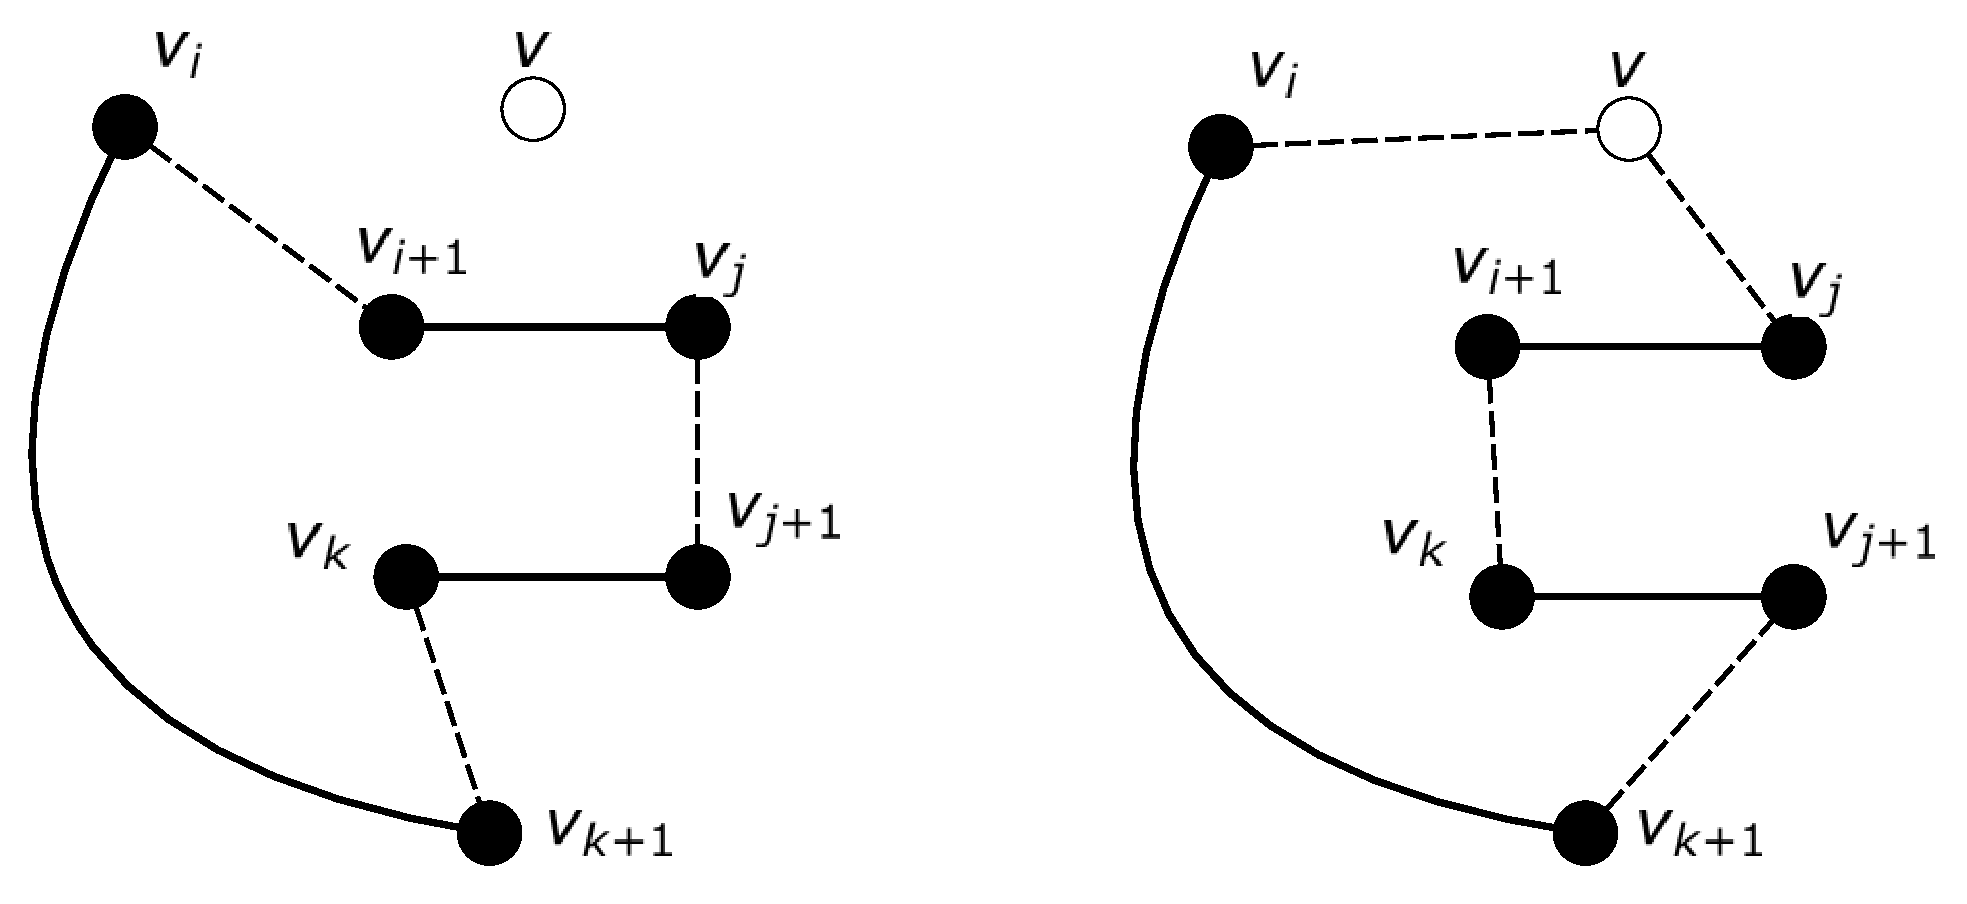
\includegraphics[width=0.7\textwidth]{Insercao-tipo-1-eps-converted-to.pdf}
		\caption{GENI - Insertion type 1 of vertex $v$ between  $v_i$ and $v_j$.}
		\label{fig:insercao1}
	\end{figure}
	
	\item \textit{Insertion type 2}: before the insertion, one verifies if $v_k \neq v_j$, $v_k \neq v_{j+1}$, $v_l \neq v_{i}$ and $v_l \neq v_{i+1}$. If it is true, so the removal of the following edges occurs: ($v_i$, $v_{i+1}$), ($v_{l-1}$, $v_l$), ($v_j$, $v_{j+1}$) and ($v_{k-1}$, $v_k$), followed by the insertion of the edges ($v_i$, $v$), ($v$, $v_j$), ($v_l$,$v_{j+1}$), ($v_{k-1}$ , $v_{l-1}$) and ($v_{i+1}$ , $v_k$ ). Thus, as in the previous insertion, the orientation of the paths ($v_{i+1}$, ..., $v_{l-1}$) and ($v_l$,..., $v_j$) are inverted to maintain the direction of the route.
	
	\begin{figure}[ht]
		\centering
		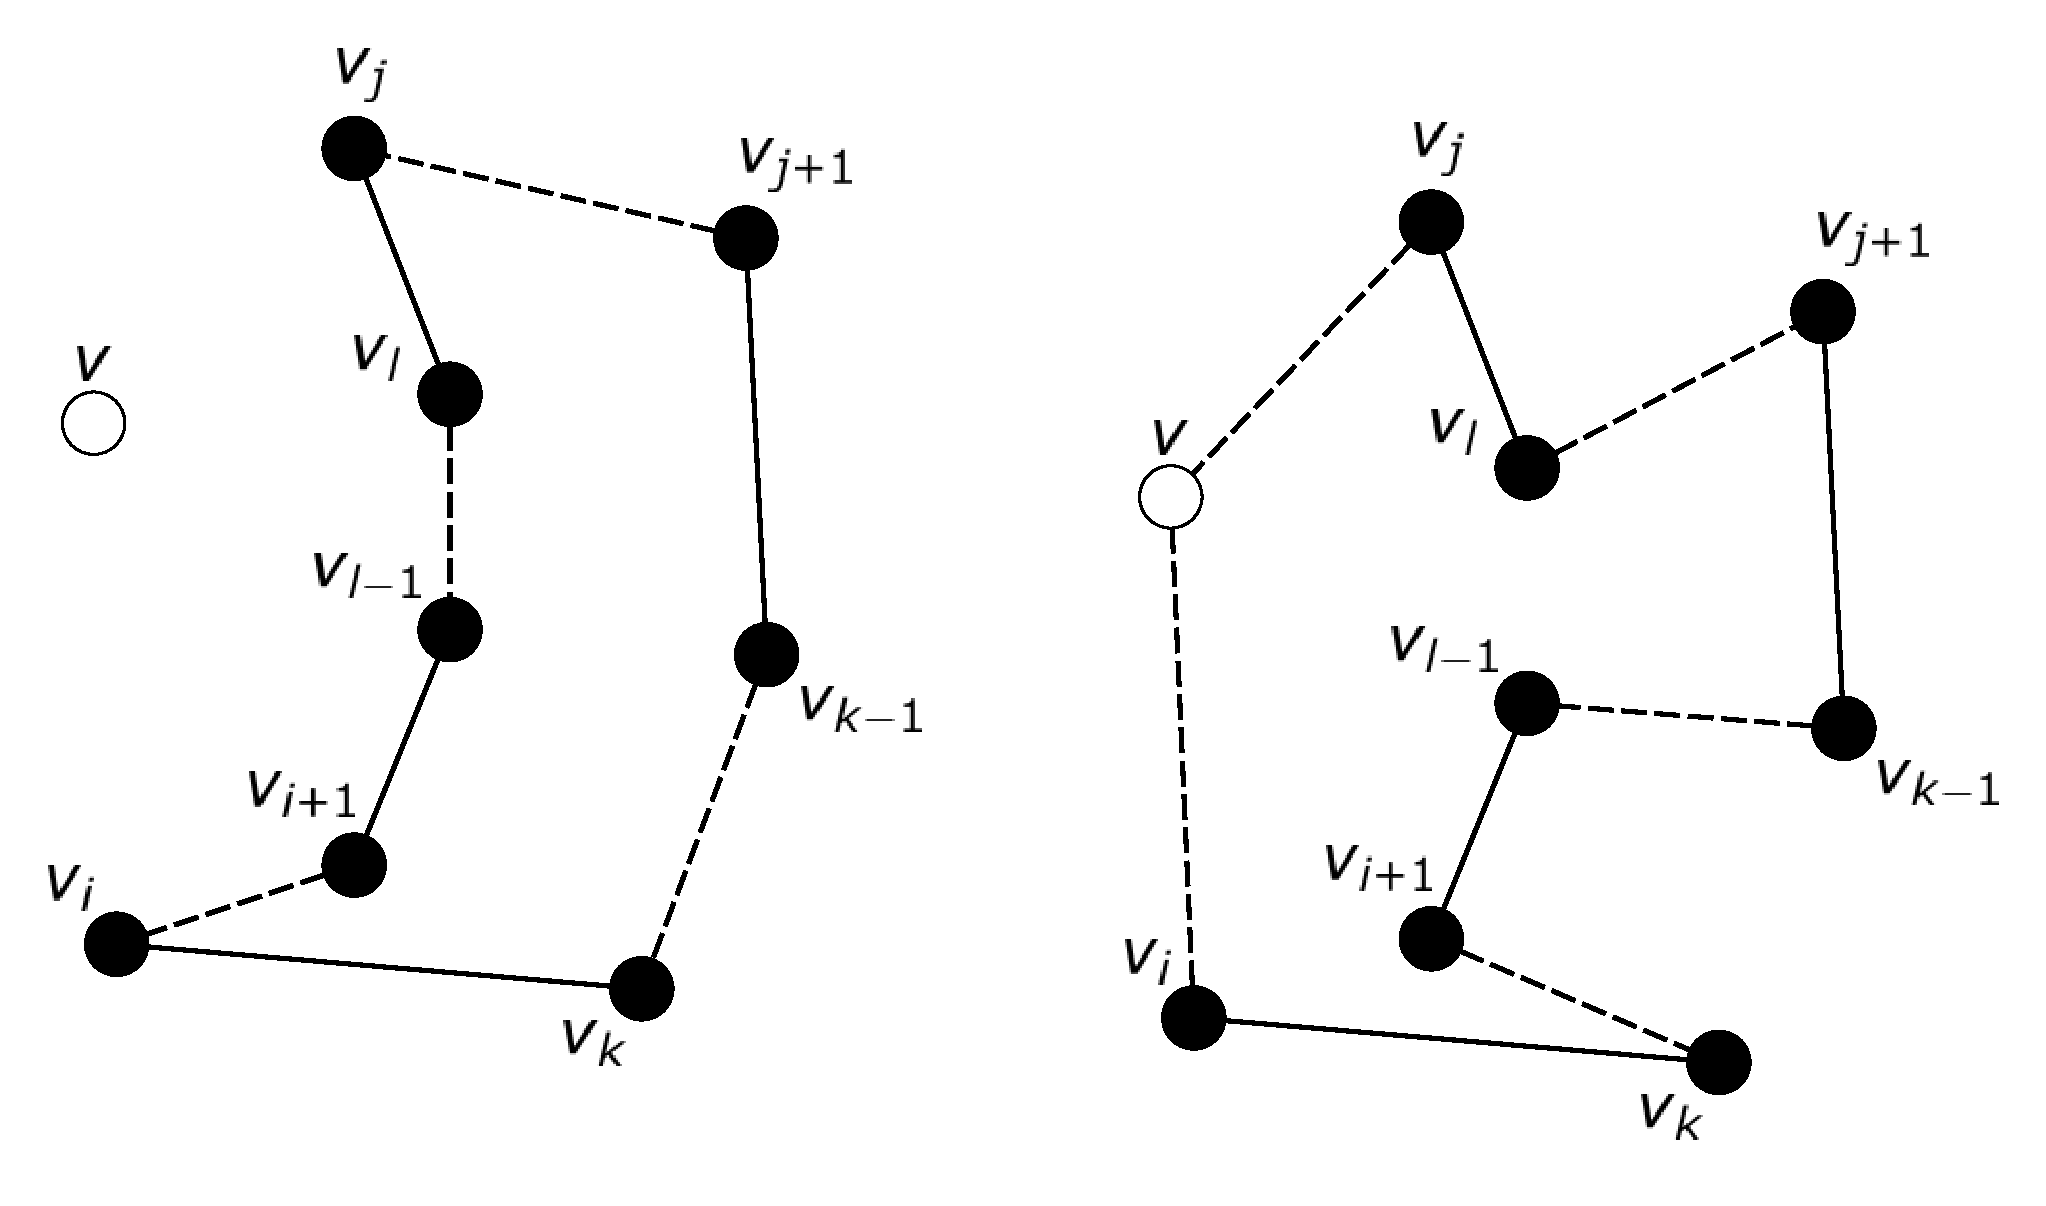
\includegraphics[width=0.7\textwidth]{insercao-tipo-2.eps}
		\caption{GENI - Insertion type 2 of the vertex $v$ between $v_i$ and $v_j$}
		\label{fig:insercao2}
	\end{figure}
	
	
\end{itemize}

In the Algorithm \ref{alg:geni}, the pseudo-code of the GENI step is illustrated, in which the method receives a partial route  $S$ and a randomly chosen vertex  $v$  to be inserted.
In line 1, the neighborhood $N_p(v)$ is created for each vertex $v$. $N_p(v)$ consists of the $p$ vertices of the route that are closest to $v$, according to the instance distance matrix. From lines 3 to 16, for every two neighbors  of $v$ and for each orientation of the route (clockwise and counter-clockwise), both types of insertion are tested. Finally, the best solution is returned on line 17.


\begin{algorithm}[ht]
	\caption{\hspace{-1mm}:GENI($S, v$)}
	\label{alg:geni}
	\begin{algorithmic}[1]			
		\STATE $N_p \gets DefineNearbyVertices(V)$;
		\STATE	$f^* \gets \infty$; $S^* \gets S$;
		\FOR{$v_i, v_j \in N_p(v), v_i \neq v_j$}
		\FOR{$orientation \in \{clockwise$,\textit{counter-clockwise}\}}
		\STATE $S' \gets insertion\_type1(v_i,v_j,S,v,orientation)$;
		\IF{$f(S') < f^*$}
		\STATE $S^* \gets S'$;
		\STATE $f^* \gets f(S^*)$;
		\ENDIF
		\STATE $S'' \gets insertion\_type2(v_i,v_j,S,v,orientation)$;
		\IF{$f(S'') < f^*$}
		\STATE $S^* \gets S''$;
		\STATE $f^* \gets f(S^*)$;
		\ENDIF
		\ENDFOR
		\ENDFOR
		\RETURN $S^*$
	\end{algorithmic}
	
\end{algorithm}

After the first step, the US step is applied to improve the  route constructed. In this step, iteratively, each one of the vertices in $S$ is removed and reinserted into $S$, using the GENI procedure. Similarly to the GENIUS construction step, the US  has two types of removal for a given vertex. Let $N_p(v)$ be the $p$ closest neighbors  of a vertex $v$, the two types of removal are detailed below and illustrated in Figures \ref{fig:remocao1} and \ref{fig:remocao2}:

\begin{itemize}
	\item \textit{US - Removal type 1}: let $v_j \in N_p(v_{i+1} )$, and let $v_k \in N_p(v_{i-1})$ be a vertex in the path \mbox{($v_{i+1}$,..., $v_{j-1}$)} for a given orientation. When removing the vertex $v_i$, the edges ($v_{i-1}, v_i $), ($v_i, v_{i+1}$), ($v_k , v_{k+1}$) and $(v_j , v_{j+1})$ are also removed. Then, the route is reconnected using the edges $(v_{i-1} , v_k )$, $(v_{i+1}, v_j )$ and $(v_{k+1} , v_{j+1}$). Moreover, the direction of the paths ($v_{i+1}$,..., $v_k$) and ($v_{k+1},..., v_j$) must be inverted.
	
	\begin{figure}[ht]
		\centering
		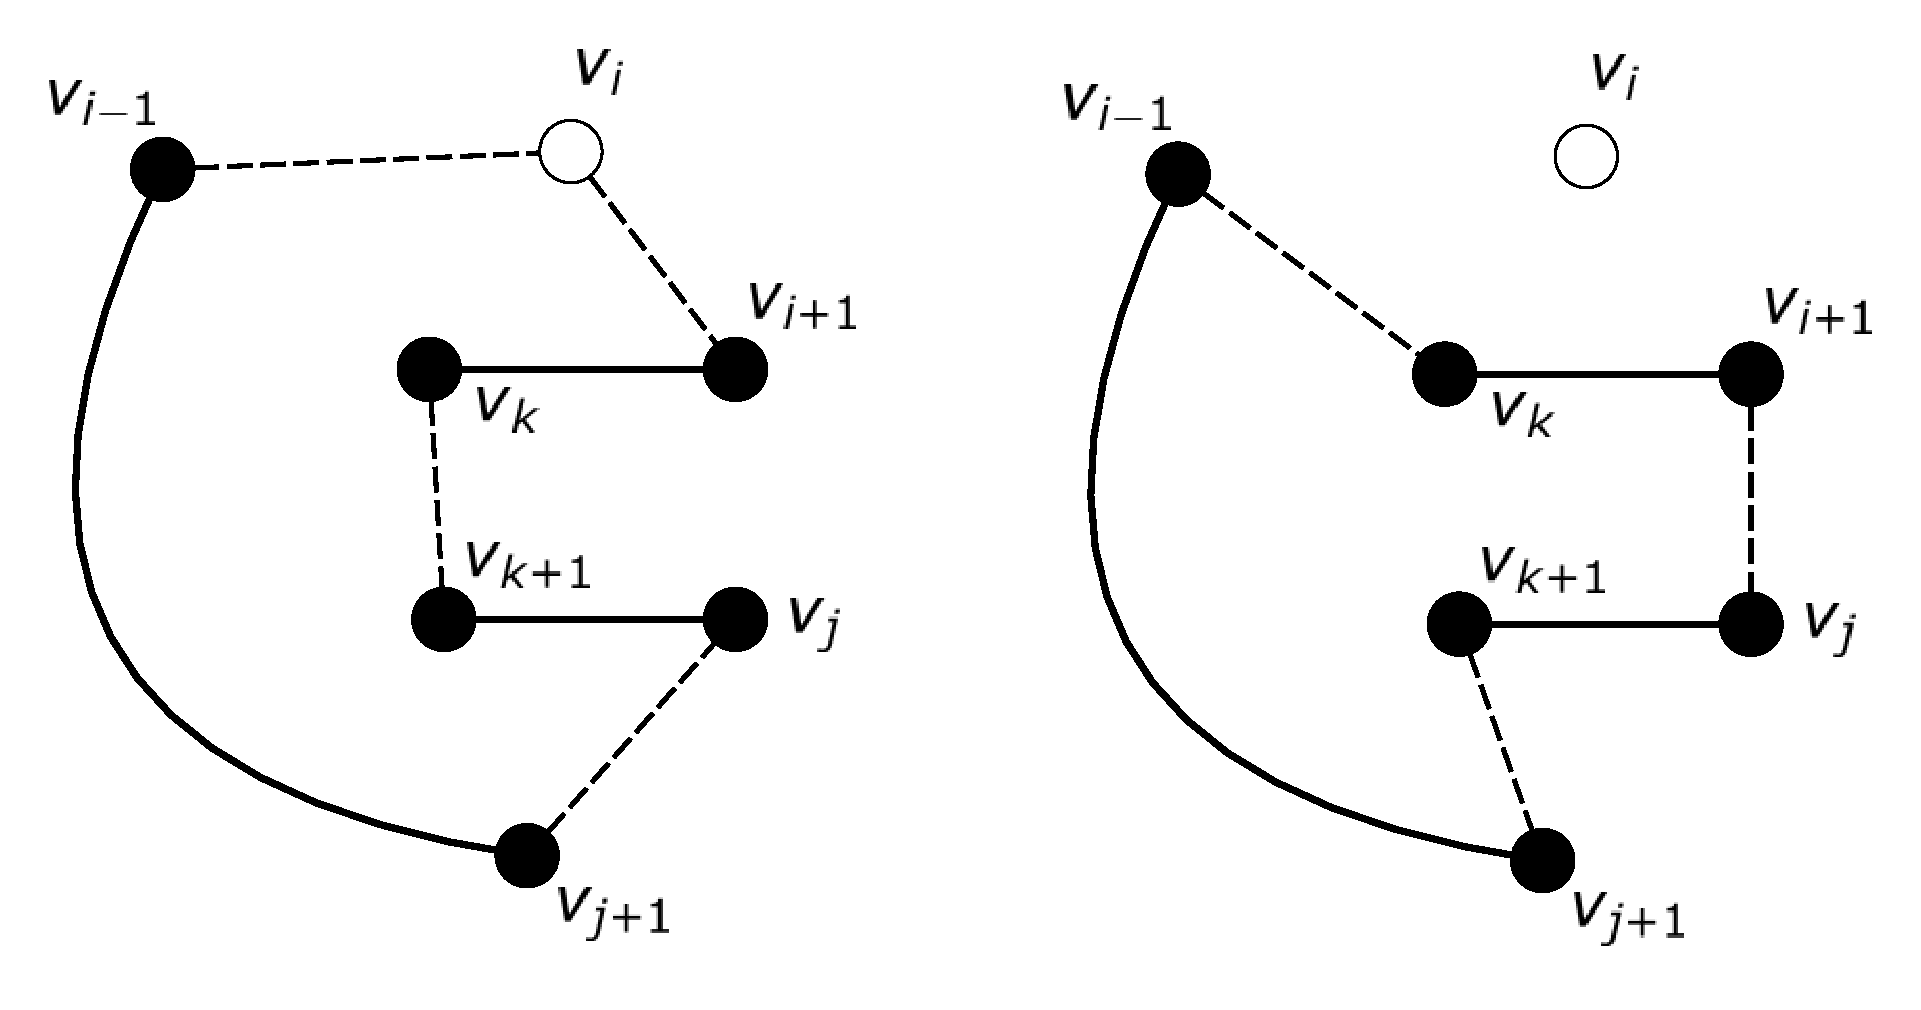
\includegraphics[width=0.7\textwidth]{remocao-tipo-1.eps}
		\caption{US - Removal type 1 of the vertex $v_i$.}
		\label{fig:remocao1}
	\end{figure}
	
	
	\item \textit{US - Removal type 2}: given an orientation of the route, consider $v_j \in N_p (v_i + 1)$ and $v_k$ a vertex in the path $(v_{j+1},...,v_{i-2})$, in which $v_k \in N_p(v_{i-1})$, and $v_l \in N_p (v_k+1)$ belongs to the path ($v_j$,...,$v_{k-1}$). When removing the vertex $v_i$ from the route, one also removes the edges $(v_{i-1} , v_i ),\-
	(v_i , v_{i+1}),\- (v_{j-1}, v_j ), \- (v_l , v_{l+1})$ and $(v_k , v_{k+1})$, and then, the connectivity of the route is re-established including the edges 
	$(v_{i-1} , v_k ),\- (v_{l+1} , v_{j-1}),\- (v_{i+1}, v_j)$ and $(v_l , v_{k+1})$. Lastly, the direction of the paths $(v_{i+1},..., v_{j-1})$ and $(v_{l+1},..., v_k)$ are inverted to ensure the orientation of the route.
	
	
	\begin{figure}[ht]
		\centering
		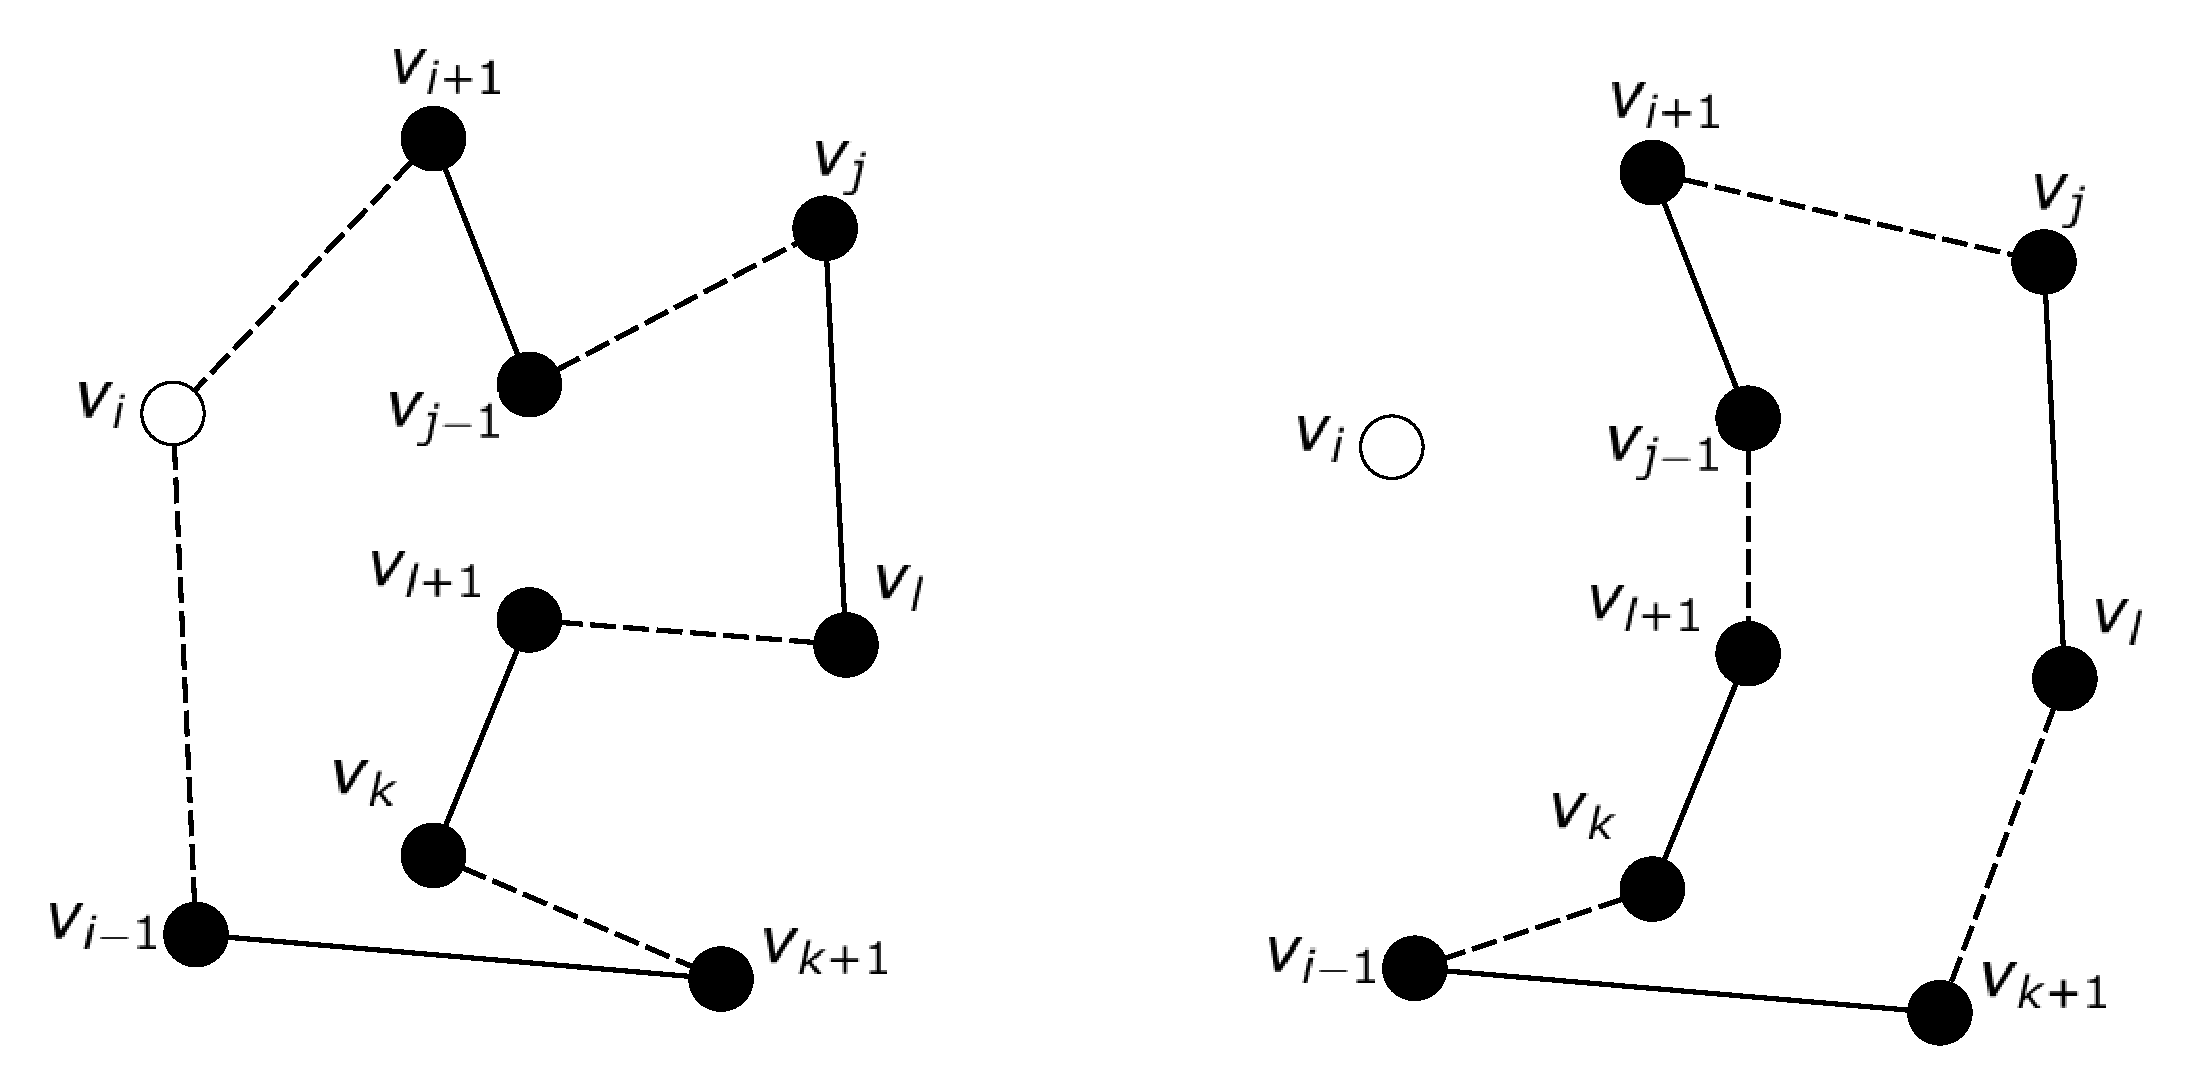
\includegraphics[width=0.7\textwidth]{remocao-tipo-2.eps}
		\caption{US - Removal type 2 of the vertex $v_i$.}
		\label{fig:remocao2}
	\end{figure}
	
\end{itemize}

The Algorithm \ref{alg:us} presents, in more detail, how the US step is performed. From lines 3 to 16, for each vertex in $S$ and each direction of the route, the two types of removal are executed. For reinserting the vertex $v$ in the route, every removal is followed by the two insertions types mentioned in the GENI step. Finally, in line 17, the route with the lowest cost is returned.

%mentioned above are tested. For each type of removal, the removal of a $v$ vertex is followed by the two types of insertions from the GENI phase, for the reinsertion of vivi into the route. Finally, on line 17, the lowest cost route found by the US phase is returned.

\begin{algorithm}[ht]
	\caption{\hspace{-1mm}:  US($S$)}
	\label{alg:us}
	\begin{algorithmic}[1]			
		\STATE $S^* \gets S$
		\STATE $f^* \gets f(S^*)$
		\FOR{\textbf{each} $v \in S$}
		\FOR{$orientation \in \{clockwise$, \textit{counter-clockwise}\}}
		\STATE $S' \gets removal\_type1(v,S,orientation)$
		\IF{$(f(S') < f^*)$}
		\STATE $S^* \gets S'$
		\STATE $f^* \gets f(S^*)$
		\ENDIF
		\STATE $S'' \gets removal\_type2(v,S,orientation)$
		\IF{$(f(S'') < f^*)$}
		\STATE $S^* \gets S''$
		\STATE $f^* \gets f(S^*)$
		\ENDIF
		\ENDFOR
		\ENDFOR
		\RETURN $S^*$
	\end{algorithmic}
	
\end{algorithm}

For the PCCTP, we have used the GENIUS procedure as follows. A partial route is generated by three vertices randomly chosen from $T$, and then, as long as the $PRIZE$ is not reached and there is any uncovered vertex $w \in W$, the following phases are performed: i) a candidate list (CL) is created containing all vertices outside the route; ii) a  restricted candidate list (RCL) is formed by the best-quality vertices from CL; iii) a vertex is selected at random from the RCL and inserted in the route using the GENI procedure; and iv) one tries to improve the route by performing the US method. The pseudo-code of the GENIUS procedure is presented in Algorithm \ref{alg:genius_PCCTP}.

A vertex is inserted into the RCL if its incremental cost is inferior to the threshold $c^{min} + (\alpha \times (c^{max} - c^{min}))$, where $c^{min}$ and $c^{max}$ are, respectively, the smallest and the largest incremental costs in CL. The greedy parameter $\alpha \in [0,1]$ indicates how greedy the heuristic is, the higher the value of $\alpha$ the greedier.

For calculating the incremental cost, we used the following greedy function, which considers the insertion of a vertex $k$ between two other vertices $i$ and $j$.

\begin{eqnarray}
g(k) = \displaystyle \min_{i,j \in V : i \neq j} \left(c_{ik} + c_{kj}  - c_{ij}\right) \label{custo_inc}
\end{eqnarray}

where $c_{ij}$, $c_{ik}$ and $c_{kj}$ are, respectively, the cost of the edges $(i,j)$, $(i,k)$ and $(k,j)$.

\begin{algorithm}[ht]
	%	\algsetup{linenosize=\scriptsize}
	\caption{\hspace{-1mm}: GENIUS($seed$,$\alpha$)}
	\label{alg:genius_PCCTP}
	%	{\footnotesize
	\begin{algorithmic}[1]
		%			\REQUIRE $seed$, $\alpha$
		\STATE $i, j, k \gets \texttt{SelectRandom}(T,seed)$;
		\STATE $S \gets \cup$ $\{i, j, k\}$;
		\STATE $CL \gets V$;
		\STATE $CL \gets CL \setminus \{i,j,k\}$
		\WHILE{$(\exists$ $t \in T$ : $t \notin S )$ \textbf{or} $(\exists$ not covered $w \in W\space)$ \textbf{or} (\textit{PRIZE} not collected) }
		\STATE $RCL \gets \texttt{setRCL}(CL, \alpha)$;
		\STATE $v \gets \texttt{SelectRandom}(RCL,seed)$;
		\STATE $S' \gets GENI(S,v)$;
		\STATE $CL \gets CL \backslash {v} $;
		\ENDWHILE
		\STATE $S'' \gets US(S')$; \textit{//route improvement}\\
		\RETURN $S''$;
	\end{algorithmic}
	%	}
\end{algorithm}



\subsection{Local search phase}

Each solution built at the constructive phase is the starting point for a local search procedure in which we try to
improve the solution. In our approach, the solution goes through a local search performed by the VND method \cite{mladenovic97}. Proposed by Mladenovi\'c and Hansen \cite{mladenovic97}, the VND is a local search metaheuristic that uses different neighborhood structures. Given an ordered list of neighborhoods, the VND starts by exploring the first neighborhood of $S$, $N^k(S)$, and if a better solution is not found, the next neighborhood $N^{(k + 1)} (S) $ is explored. Otherwise, it returns to the first neighborhood on the list. The algorithm stops when all neighborhood structures are explored, returning the best solution found. 

%In this work, we have used the VND instead of conventional the VND, where there is no fixed sequence of neighborhoods, because they are sorted on each application of the local search.

The VND is detailed in the pseudo-code of Algorithm \ref{alg:vnd}. From lines 2 to 10, it tries the next neighborhood if the current solution is not improved. Otherwise, the  local optimal solution for the current neighborhood is obtained, and $k$ is set to 1 so that the loop restarts for the newly accepted solution. When none of the neighbors are able to improve $S$, i.e., $k > k_{max}$, the best current solution is returned.

For the VND, we used  the following 15 neighborhood structures based on classical movements for the TSP as \textit{swap} and \textit{shift}, and heuristics as GENIUS and Cheapest Insertion. In particular, 
one of them, the \textit{double\_remove\_\-simple\-\_insert\-\_cheapest}, is proposed in this work. 


Of the 15 neighborhood structures used, ten are intra-route:

%{\footnotesize
	\begin{enumerate}
		\item {\it shift}: changes the position of a vertex within the route;
		\item {\it swap}: swaps the position of two vertices in the route;
		
		\item {\it or-opt}: movement similar to \textit{shift}, but the position of $n$ vertices is changed;%foi usando n=2 no código
		\item {\it 2-opt}: removes two non-adjacent edges of the solution and inserts two new ones to keep the single cycle;
		\item {\it 3-opt}: removes three non-adjacent edges and inserts three new ones, similar to {\it 2-opt};
		\item {\it remove\_simple\_re\_insert\_cheapest}: removes a vertex and reinserts it via the cheaper insertion;
		\item {\it remove\_simple\_re\_insert\_genius}: removes a vertex and reinsert it via GENIUS method;
		\item {\it remove\_genius\_re\_insert\_cheapest}: Removes a vertex using a GENIUS removal method and inserts using lower cost criteria between adjacent vertices;
		\item {\it remove\_genius\_re\_insert\_genius}: removes and reinsert a vertex of the route using GENIUS; 
		\item {\it remove\_cheapest\_re\_insert\_genius}: removes using chea\-per insertion criteria and re-enter via GENIUS;
	\end{enumerate}
%}
and five of them are extra-route:
%{\small
%{\footnotesize
	\begin{enumerate}
		
		
		\item {\it double\_remove\_simple\_insert\_cheapest}: tries to replace two vertices with a single one that does not belong to the solution;
		\item {\it remove\_simple\_insert\_cheapest}: replaces a vertex of the route with an outside vertex, inserting via cheaper insertion;
		\item {\it remove\_simple\_insert\_genius}: replaces a vertex  of the route with an outside vertex, inserting via GENIUS;
		\item {\it remove\_genius\_insert\_genius}: replaces a vertex  of the route with an outside vertex, by removing and inserting via GENIUS; and
		\item {\it remove\_genius\_insert\_cheapest}: removes a vertex from the solution via GENIUS and inserts a new one via cheapest insertion.
	\end{enumerate}
	%}
%}
It is important to remark that only feasible movements are performed. 




% From the algorithm, we can see that the counter n is
%increased by one to try next neighbor if the current solution
%is not improved. Otherwise, the better solution is found, and
%n is set to 1 so that the cycle restarts for the newly accepted
%solution. When none of the neighbors make an improvement
%in succession, which implies n > k, the algorithm returns
%the current solution. T
%
% Lines 1 and 2 define the number of neighborhoods to be explored. From lines 3 to 11, iteratively, the best neighbor $S'$ is selected in each neighborhood of SS (line 4); it is checked whether S?S? is better than SS (line 5); if true, $S'$ becomes the best current VND solution (line 6) and the algorithm returns to the first neighborhood (line 7); otherwise, the algorithm advances to the next neighborhood (line 9). After exploring all the neighborhoods, without finding a better solution than SS, SS is returned as the final VND solution.

\begin{algorithm}
	\caption{\hspace{-1mm}: VND($S$).}
	\label{alg:vnd}
	\begin{algorithmic}[1]		
	%	\STATE  Set a random order for the neighborhood structures in $N$	
		\STATE $k \gets 1$
		\WHILE {$k \leq k\_max$}
		\STATE $S' \gets firstImprovingSolution(N^{(k)}(S))$;
		\IF{\textit{S' is better than S}}
		\STATE $S \gets S'$;
		\STATE $k \gets 1$;
		\ELSE
		\STATE $k \gets k + 1$;
		\ENDIF
		\ENDWHILE
		\RETURN $S$
	\end{algorithmic}
	
\end{algorithm}

\subsection{R-GRASP heuristic}

%A heuristic based on the GRASP metaheuristic is proposed to solve the PCCTP. This heuristic uses an adaptation of the GENIUS heuristic \cite{genius} for generating an initial solution, and the VND \cite{mladenovic97} as an improvement method. 

In the construction phase of the R-GRASP, a preliminary computational experience showed that no value of $\alpha$ always produced the best results. Therefore, we decided to devise a reactive version of the GRASP proposed by Prais and Ribeiro \cite{prais2000reactive}, in which  $\alpha$ is taken at random from a set of discrete
values. Initially, all $\alpha$ values have the same probability of being chosen. In the iterative process, one keeps the value of the solutions obtained for each value of $\alpha$. After a certain number of iterations, the probabilities are updated. Those corresponding to values of  which have produced good solutions are increased and, conversely, those corresponding to values producing low-quality solutions are decreased. The Reactive GRASP (R-GRASP) is described in Algorithm \ref{alg:grasp}, and the value of $\beta$ is fixed at 10, as in \cite{prais2000reactive}.

\begin{algorithm}[!h]
	\caption{\hspace{-1mm}:  R-GRASP($maxIt$, $seed$,  $\beta=10$)}
	\label{alg:grasp}
	{\footnotesize
		\begin{algorithmic}[1]	
		    \STATE $\mathcal{D} \gets \{0.1,0.2 \ldots ,0.9\}$ \hfill\COMMENT{\texttt{set of possible values for $\alpha$}}
		    \STATE $n_{\alpha^*} \gets 0$ \hfill \COMMENT{\texttt{number of iterations with $\alpha^*, \quad \forall \alpha^* \in \mathcal{D}$}}
		    \STATE $Sum_{\alpha^*} \gets 0$ \hfill \COMMENT{\texttt{sum of values of solutions obtained with $\alpha^*$}}
		    \STATE $p_{\alpha=\frac{1}{|\mathcal{D}|}} \quad \forall \alpha \in \mathcal{D}$
			\STATE $S_{best} \gets \infty$; $S_{worst} \gets 0$; $it \gets 0$
			\WHILE{($it < maxIt$)}
		%	\STATE $\alpha^* \gets RandomSelect(p, D)$
		    \STATE Choose $\alpha^*$ from $\mathcal{D}$ with probability of $p_{\alpha}$
			\STATE $S \gets GENIUS(seed, \alpha^*)$ 
			\STATE $S' \gets VND(S)$
			\IF{$S' < S_{best}$}
			\STATE $S_{best} \gets S'$
			\ENDIF
			\IF{$S' > S_{worst}$}
            \STATE $S_{worst} \gets S'$
            \ENDIF
            \STATE $sum_{\alpha^*} \gets sum_{\alpha^*} + S'$
			\STATE $n_{\alpha^*} \gets n_{\alpha^*} + 1$
            \IF{$mod(it,15)==0$}
            \STATE $mean_{\alpha} \gets \frac{sum_{\alpha^*}}{n_{\alpha^*}}$
            \STATE $eval_{\alpha} \gets \left( \frac{S_{worst} - mean_{\alpha}}{S_{worst} - S_{best}} \right)^\beta \quad \forall \alpha \in D$
            \STATE $p_{\alpha} \gets \frac{eval_{\alpha}}{\left( \sum_{\alpha' \in D} eval_{\alpha'}\right)}\qquad \forall \alpha \in D$
            \ENDIF
            
			\STATE $it \gets it + 1$;
			\ENDWHILE
			\RETURN $S_{best}$;
		\end{algorithmic}
	}
\end{algorithm}	

From lines 1 to 5, some variables are initialized and, from
In line 1, some variables are initialized and, from lines 6 to 24, while the maximum number of iterations $maxIt$ is not reached, the following instructions are executed. In line 7 $\alpha^*$ is chosen at random from set $\mathcal{D}$ with probability of $p_{\alpha}$.
In lines 8 and 9, at each iteration, the solution construction and local search procedures are performed. An initial   solution $S$ is built using the GENIUS method, adapted for the PCCTP, and then the local search is performed employing the VND method. At the end of the local search, the VND returns a  solution value $S'$ that is compared to the best current solution  value (line 10). If  $S'$  is better than $S_{best}$, then the best solution value is updated (line 11). From lines 13 to 15, the worst solution value found so far is updated. From lines 18 to 22,  the probabilities are updated every 15 GRASP iterations.
Finally, in line 25, the best solution value obtained over all iterations is returned.


\section{Computational results}
\label{sec:results}

In this section, it is presented the computational experiments performed with the R-GRASP, the ILS-RDM-CI, and the mathematical formulations. All strategies presented were implemented in C programming language and compiled with GCC version 4.7.0. All experiments were carried out on a 3.2GHz $Intel Core^{TM}$ i5 CPU under Linux Fedora 15 operational system. As regards the MIP solver, Gurobi optimizer \cite{gurobi} was used disabling its preprocessing heuristics, cuts,
and the parallel mode set to none. We remark that the original source code of the ILS-RDM-CI heuristic was
kindly provided by its author Silva \cite{silva2009problema} and used in our computational experiments.


\subsection{Instances}

The instances used in this work were proposed by Silva \cite{silva2009problema}, and consist of 144 test problems adapted from the traveling salesman problem (TSP) available at the TSPLIB repository \cite{reinelt1991tsplib}. To prevent any instance of the PCCTP from becoming an instance of the covering tour problem (CTP), the \textit{PRIZE} is never satisfied with the collection of only the prizes associated with the mandatory vertices $T$.


These instances were named according to their original name in the TSPLIB, adding additional information about the subsets $R$, $T$, $W$ and the percentage of prize to be collected, concerning the total available prize. For example, the instance \textit{brazil58\_R18\_T20\_W20\_25} has the following characteristics: 58 vertices in total; 18 optional vertices $R$; 20 mandatory vertices $T$; 20 vertices to be covered $W$; and 25\% of the total instance prize must be collected. These instances were made public in the Mendeley repository (see \cite{pcctp-data}).


%The same 144 instances described in \cite{silva2009problema} were used to perform the
%experiments, which are derived from the classical TSP benchmark available at the TSPLIB repository \cite{reinelt1991tsplib}.

\subsection{Mathematical formulations}

This section presents an unprecedented comparison between the two formulations present in the literature, Flow \cite{lyra2004problema} and Multi-flow \cite{silva2009problema}, since the Flow formulation has never been tested before in Silva's  instances \cite{silva2009problema}. Then, the formulation with the best results will be compared with the performance of the proposed heuristic.


Table \ref{tab:models} presents the results obtained by executing these formulations. The first column refers to the name of the instances. From the second column, the solution, the best bound and the time spent (in seconds) by each formulation are presented. For clarity and ease of reading purposes, it was decided to present only the 50 instances that yield the biggest differences of performance between the formulations, either in solution quality or CPU time. The complete results are available in a Mendeley repository (see \cite{pcctp-data-complete}).

The fields with ``- '' indicate that, due to the time exceeded by one hour of processing, or problems related to lack of memory, it was not possible to solve the respective instance. The values in bold indicate the best results in processing time and the best solution found.


\begin{table}[!htb]
	\centering
	\caption{Results for the mathematical formulations.}
	\label{tab:models}
		\begin{tabular}{lr@{\hspace{0.5\tabcolsep}}r@{\hspace{\tabcolsep}}r@{\hspace{3.0\tabcolsep}}r@{\hspace{0.3\tabcolsep}}r@{\hspace{0.5\tabcolsep}}r}
			\hline \hline
		& \multicolumn{3}{c}{Flow}              & \multicolumn{3}{c}{Multi-flow}                                 \\
		\cline{2-7}
		Instance &
		\multicolumn{1}{c}{Sol} &
		\multicolumn{1}{c}{\begin{tabular}[c]{@{}c@{}}Best \\ Bound\end{tabular}} &
		\multicolumn{1}{c}{T (s)} &
		\multicolumn{1}{c}{Sol} &
		\multicolumn{1}{c}{\begin{tabular}[c]{@{}c@{}}Best \\ Bound\end{tabular}} &
		\multicolumn{1}{c}{T (s)} \\
		\hline
		bier127\_R43\_T42\_W42\_75  & 251062                & 83756 & 3600.0 & - & 96950                 & 3600.0          \\
		brg180\_R36\_T36\_W108\_25  & 142850                & 180   & 3600.0 & - & - & 3600.0          \\
		pr76\_R14\_T46\_W16\_75     & 219818                & 66871 & 3600.0 & \textbf{90862}        & 90862                 & \textbf{523.3}  \\
		lin105\_R21\_T63\_W21\_50   & 58498                 & 6833  & 3600.0 & - & 11573                 & 3600.0          \\
		pr107\_R35\_T36\_W36\_75    & 57482                 & 20295 & 3600.0 & - & 37040                 & 3600.0          \\
		pr144\_R28\_T29\_W87\_50    & 82642                 & 11123 & 3600.0 & \textbf{30294}        & 30294                 & \textbf{408.0}  \\
		bier127\_R24\_T26\_W77\_50  & 125855                & 62064 & 3600.0 & \textbf{74745}        & 74745                 & \textbf{495.2}  \\
		kroA100\_R34\_T33\_W33\_75  & 47550                 & 10137 & 3600.0 & - & 14549                 & 3600.0          \\
		kroB200\_R40\_T40\_W120\_50 & 45214                 & 7306  & 3600.0 & - & -            & 3600.0          \\
		gr96\_R18\_T58\_W20\_25     & - & 33028 & 3600.0 & \textbf{42746}        & 42746                 & \textbf{1670.9} \\
		pr76\_R24\_T26\_W26\_50     & 116859                & 52704 & 3600.0 & \textbf{74539}        & 74539                 & \textbf{1012.3} \\
		gr96\_R32\_T32\_W32\_50     & 74785                 & 28599 & 3600.0 & \textbf{35461}        & 35461                 & \textbf{993.1}  \\
		kroC100\_R20\_T60\_W20\_25  & 45872                 & 12478 & 3600.0 & \textbf{16785}        & 16785                 & \textbf{3369.8} \\
		pr136\_R26\_T28\_W82\_25    & 76646                 & 34449 & 3600.0 & \textbf{47620}        & 47620                 & \textbf{243.8}  \\
		kroE100\_R34\_T33\_W33\_75  & 27385                 & 10255 & 3600.0 & - & 14202                 & 3600.0          \\
		kroC100\_R34\_T33\_W33\_50  & 40281                 & 8004  & 3600.0 & \textbf{13235}        & 13235                 & \textbf{1796.3} \\
		pr124\_R24\_T25\_W75\_75    & 62995                 & 15408 & 3600.0 & \textbf{36719}        & 33585                 & 3600.0          \\
		kroB100\_R34\_T33\_W33\_75  & 25197                 & 11115 & 3600.0 & - & 14301                 & 3600.0          \\
		kroB100\_R34\_T33\_W33\_50  & 24846                 & 9217  & 3600.0 & - & 12506                 & 3600.0          \\
		pr152\_R29\_T31\_W92\_75    & 70971                 & 19577 & 3600.0 & \textbf{49167}        & 40798                 & 3600.0          \\
		u159\_R31\_T32\_W96\_50     & 47566                 & 24433 & 3600.0 & \textbf{28613}        & 28613                 & \textbf{606.4}  \\
		kroB150\_R30\_T30\_W90\_25  & 18533                 & 5384  & 3600.0 & - & 7196                  & 3600.0          \\
		kroE100\_R20\_T60\_W20\_25  & - & 12235 & 3600.0 & \textbf{17199}        & 17199                 & \textbf{3091.3} \\
		d198\_R39\_T40\_W119\_25    & 14140                 & 6432  & 3600.0 & - & 10911                 & 3600.0          \\
		gr120\_R40\_T40\_W40\_25    & 17438                 & 3514  & 3600.0 & \textbf{4301}         & 4301                  & \textbf{1929.8} \\
		pr107\_R20\_T22\_W65\_50    & 47333                 & 23618 & 3600.0 & \textbf{35869}        & 35869                 & \textbf{65.7}   \\
		lin105\_R35\_T35\_W35\_75   & - & 6340  & 3600.0 & \textbf{11090}        & 10549                 & 3600.0          \\
		rd100\_R34\_T33\_W33\_25    & 15716                 & 4168  & 3600.0 & \textbf{5970}         & 4989                  & 3600.0          \\
		brazil58\_R11\_T35\_W12\_50 & 32029                 & 16750 & 3600.0 & \textbf{23312}        & 23312                 & \textbf{109.6}  \\
		ch150\_R30\_T30\_W90\_75    & 10981                 & 3876  & 3600.0 & \textbf{4292}         & 4292                  & \textbf{513.7}  \\
		ch130\_R26\_T78\_W26\_75    & 5443                  & 3352  & 3600.0 & - & -                     & 3600.0          \\
		gr120\_R24\_T24\_W72\_75    & 9702                  & 3563  & 3600.0 & \textbf{4275}         & 4275                  & \textbf{139.7}  \\
		si175\_R35\_T35\_W105\_25   & 9941                  & 3593  & 3600.0 & \textbf{4845}         & 4845                  & \textbf{1960.3} \\
		gr96\_R18\_T20\_W58\_75     & 34379                 & 24392 & 3600.0 & \textbf{30015}        & 30015                 & \textbf{467.1}  \\
		ch130\_R26\_T26\_W78\_50    & - & 3408  & 3600.0 & \textbf{4139}         & 4139                  & \textbf{296.0}  \\
		kroC100\_R20\_T20\_W60\_75  & 15900                 & 7078  & 3600.0 & \textbf{12582}        & 12582                 & \textbf{78.4}   \\
		rat195\_R39\_T39\_W117\_50  & 2345                  & 1034  & 3600.0 & - & 1147                  & 3600.0          \\
		lin105\_R21\_T21\_W63\_25   & 11121                 & 4853  & 3600.0 & \textbf{8893}         & 8893                  & \textbf{90.9}   \\
		brazil58\_R18\_T20\_W20\_25 & 21198                 & 15786 & 3600.0 & \textbf{19417}        & 19417                 & \textbf{798.9}  \\
		kroE100\_R20\_T20\_W60\_50  & 12260                 & 6632  & 3600.0 & \textbf{10586}        & 10586                 & \textbf{551.7}  \\
		eil101\_R19\_T61\_W21\_50   & 1547                  & 451   & 3600.0 & - & 503                   & 3600.0          \\
		gr137\_R26\_T28\_W83\_25    & \textbf{59114}        & 25048 & 3600.0 & 60630                 & 39167                 & 3600.0          \\
		rd100\_R20\_T20\_W60\_75    & 6705                  & 4834  & 3600.0 & \textbf{5421}         & 5421                  & \textbf{143.4}  \\
		kroA100\_R20\_T20\_W60\_25  & 11980                 & 5566  & 3600.0 & \textbf{10848}        & 10848                 & \textbf{104.6}  \\
		eil101\_R33\_T34\_W34\_75   & 1367                  & 407   & 3600.0 & \textbf{462}          & 462                   & 3600.0          \\
		hk48\_R9\_T29\_W10\_25      & 10557                 & 8557  & 3600.0 & \textbf{9708}         & 9708                  & \textbf{50.5}   \\
		gr48\_R9\_T29\_W10\_75      & 5135                  & 4097  & 3600.0 & \textbf{4415}         & 4415                  & \textbf{0.4}    \\
		rat99\_R19\_T20\_W60\_25    & 1362                  & 737   & 3600.0 & \textbf{792}          & 792                   & \textbf{12.8}   \\
		pr76\_R14\_T16\_W46\_25     & 66533                 & 50625 & 3600.0 & \textbf{66007}        & 66007                 & \textbf{10.4}   \\
		kroA150\_R30\_T30\_W90\_50  & \textbf{19405}        & 6544  & 3600.0 & 19898                 & 9778                  & 3600.0   \\
		\hline      
	\end{tabular}
\end{table}

From Table \ref{tab:models}, it can be seen that, among the most prominent results, it is shown that the Multi-flow formulation \cite{silva2009problema}  outperforms the Flow formulation  \cite{lyra2004problema} in terms of processing time and quality of the solution obtained. Considering all the 144 instances and the solution quality achieved, the Multi-Flow model wins in 46, ties in 82, and loses in 16 instances. Concerning the CPU time spent, the formulation of Silva \cite{silva2009problema} is faster for 48 instances, slower for just one instance, and ties in 95 cases, where the time limit is reached in both models.


\subsection{Heuristics}

The GRASP heuristic includes a probabilistic behavior by setting, in the construction phase, a restricted candidate list ($RCL$) with the best candidates. In our proposal, the $RCL$ is composed of all elements \(v \in LC\) whose incremental cost is inferior to $c^{min} + \alpha^* (c^{max} - c^{min})$. 

As we made use of a reactive GRASP, there was no need to tune the $\alpha$ parameter, so the tuning experiments were made just for the $maxIt$ parameter. We have conducted the tuning experiment on a subset of 37 instances that best represent the whole set of instances. By running ten executions for each one of the 37 instances, and  for each value of $maxIt \in \{50,60,70,80,90,100\}$, we realized that $maxIt=70$ fits better our approach.


Next, we conducted experiments with the remaining 107 instances, which were not used for tuning. Both approached were run ten times with the same ten different seeds, and the results are presented in  Table \ref{tab:comp}. As in the section above, we have decided to present only the 50 instances in which R-GRASP had the greatest impact over ILS-RDM-CI, and the complete results are available in a Mendeley repository (see \cite{pcctp-data-complete}).

In Table \ref{tab:comp}, the first column indicates the name of the instance, and the results obtained by the MIP solver Gurobi through the formulation of  Silva \cite{silva2009problema}, are presented on the second and third columns. The remaining columns show for each method, respectively, the best solution, the average solution, and the average time spent. The last column shows the  percentage time difference between the compared heuristics according to equation (\ref{eq:time}). Moreover, the symbol ``-'' indicates that no solution was found by Gurobi within a one-hour CPU time, and the best results are bold-faced.



{\footnotesize
	\begin{equation}
	\label{eq:time}
	Diff_{T} = 100*\frac{(T_{grasp}- T_{ils})}{T_{ils}}
	\end{equation}
}
\begin{table}[!ht]
\centering
\caption{Comparison between R-GRASP and ILS-RDM-CI heuristics}
\label{tab:comp}
{\footnotesize \centering
\begin{tabular}{lcrrrrrrr}
\hline
\hline
 & \multicolumn{1}{l}{} & \multicolumn{3}{c}{ILS-RDM-CI} & \multicolumn{4}{c}{R-GRASP} \\
 \cline{2-9}
Instance & \multicolumn{1}{l}{Multi-flow} & \multicolumn{1}{l}{\begin{tabular}[c]{@{}l@{}}Best \\ Sol.\end{tabular}} & \multicolumn{1}{l}{\begin{tabular}[c]{@{}l@{}}Avg.\\ Sol.\end{tabular}} & \multicolumn{1}{l}{\begin{tabular}[c]{@{}l@{}}Avg.\\ T (s)\end{tabular}} & \multicolumn{1}{l}{\begin{tabular}[c]{@{}l@{}}Best\\ Sol.\end{tabular}} & \multicolumn{1}{l}{\begin{tabular}[c]{@{}l@{}}Avg.\\ Sol.\end{tabular}} & \multicolumn{1}{l}{\begin{tabular}[c]{@{}l@{}}Avg.\\ T (s)\end{tabular}} & \multicolumn{1}{l}{\begin{tabular}[c]{@{}l@{}}$Diff_{T}$ \end{tabular}} \\
\hline
pr226\_R76\_T75\_W75\_25 & - & 40994 & 41014.00 & 1627.04 & 40994 & \textbf{40994.00} & \textbf{4.37} & -99.70 \\
rd400\_R136\_T132\_W132\_75 & - & 35465 & 36107.90 & 1497.27 & 35465 & \textbf{35465.00} & \textbf{6.30} & -99.50 \\
pr124\_R42\_T41\_W41\_25 & - & 61068 & 61077.70 & 2463.89 & 61068 & \textbf{61068.00} & \textbf{15.24} & -99.30 \\
lin318\_R108\_T105\_W105\_50 & 3571 & 3571 & 3571.00 & 8.89 & 3571 & 3571.00 & \textbf{0.05} & -99.30 \\
kroA150\_R50\_T50\_W50\_25 & 2650 & 2650 & 2650.00 & 27.96 & 2650 & 2650.00 & \textbf{0.19} & -99.20 \\
gr229\_R77\_T76\_W76\_75 & 19417 & 19417 & 19417.00 & 55.64 & 19417 & 19417.00 & \textbf{0.44} & -99.10 \\
pr299\_R101\_T99\_W99\_75 & 35869 & 35869 & 35869.00 & 22.79 & 35869 & 35869.00 & \textbf{0.17} & -99.10 \\
d198\_R66\_T66\_W66\_75 & 36719 & 34359 & 34359.00 & 201.94 & 34359 & 34359.00 & \textbf{1.52} & -99.10 \\
kroB150\_R50\_T50\_W50\_50 & 5970 & 5552 & 5552.00 & 169.72 & 5552 & 5552.00 & \textbf{1.32} & -99.10 \\
ts225\_R75\_T75\_W75\_75 & 792 & 792 & 792.00 & 74.65 & 792 & 792.00 & \textbf{0.65} & -99.00 \\
pr299\_R59\_T180\_W60\_25 & 13235 & 13235 & 13238.40 & 821.52 & 13235 & \textbf{13235.00} & \textbf{7.55} & -98.90 \\
gil262\_R88\_T87\_W87\_50 & 863 & 847 & 847.00 & 217.58 & 847 & 847.00 & \textbf{2.09} & -98.90 \\
a280\_R94\_T93\_W93\_25 & 248 & 248 & 248.00 & 3.68 & 248 & 248.00 & \textbf{0.04} & -98.80 \\
lin318\_R63\_T191\_W64\_75 & 338 & 338 & 338.00 & 122.08 & 338 & 338.00 & \textbf{1.26} & -98.80 \\
si175\_R59\_T58\_W58\_75 & 5421 & 5421 & 5421.00 & 35.57 & 5421 & 5421.00 & \textbf{0.37} & -98.80 \\
tsp225\_R75\_T75\_W75\_50 & 273 & 273 & 273.00 & 67.94 & 273 & 273.00 & \textbf{0.75} & -98.70 \\
pr299\_R59\_T60\_W180\_50 & 4275 & 4275 & 4275.00 & 57.88 & 4275 & 4275.00 & \textbf{0.63} & -98.70 \\
pr144\_R48\_T48\_W48\_75 & 90862 & 90862 & 90862.00 & 90.38 & 90862 & 90862.00 & \textbf{1.09} & -98.60 \\
rat195\_R39\_T39\_W117\_50 & - & 1199 & 1202.80 & 3308.10 & 1199 & \textbf{1199.00} & \textbf{42.48} & -98.50 \\
gil262\_R51\_T158\_W53\_75 & 60630 & 39305 & 39305.00 & 101.86 & 39305 & 39305.00 & \textbf{1.34} & -98.50 \\
gr137\_R45\_T46\_W46\_50 & - & 10916 & 10918.30 & 1187.35 & 10916 & \textbf{10916.00} & \textbf{15.92} & -98.40 \\
si175\_R35\_T35\_W105\_25 & 6916 & 6916 & 6916.00 & 115.10 & 6916 & 6916.00 & \textbf{1.69} & -98.30 \\
pr264\_R88\_T88\_W88\_50 & 4301 & 4301 & 4301.00 & 82.83 & 4301 & 4301.00 & \textbf{1.23} & -98.30 \\
kroB200\_R40\_T40\_W120\_50 & 356 & 356 & 356.00 & 241.04 & 356 & 356.00 & \textbf{3.90} & -98.10 \\
rat195\_R39\_T117\_W39\_75 & - & 4383 & 4385.50 & 1680.15 & 4383 & \textbf{4383.00} & \textbf{30.41} & -97.90 \\
kroB150\_R30\_T90\_W30\_75 & 12582 & 12582 & 12582.00 & 14.77 & 12582 & 12582.00 & \textbf{0.27} & -97.90 \\
gr229\_R45\_T138\_W46\_50 & - & 35442 & 35442.00 & 1721.60 & 35442 & 35442.00 & \textbf{31.58} & -97.90 \\
ts225\_R45\_T135\_W45\_50 & - & 550 & 551.00 & 552.07 & 550 & \textbf{550.00} & \textbf{10.66} & -97.80 \\
kroA200\_R68\_T66\_W66\_50 & 419 & 419 & 419.00 & 10.82 & 419 & 419.00 & \textbf{0.20} & -97.80 \\
bier127\_R43\_T42\_W42\_75 & 554 & 554 & 554.00 & 92.55 & 554 & 554.00 & \textbf{1.73} & -97.80 \\
eil101\_R33\_T34\_W34\_75 & 4845 & 4845 & 4863.60 & 4252.27 & 4845 & \textbf{4847.40} & \textbf{84.02} & -97.70 \\
pr264\_R52\_T159\_W53\_75 & 3524 & 3524 & 3524.00 & 3.31 & 3524 & 3524.00 & \textbf{0.07} & -97.60 \\
brg180\_R36\_T36\_W108\_25 & - & 15197 & 15201.00 & 2460.12 & 15197 & \textbf{15197.00} & \textbf{52.49} & -97.50 \\
gr229\_R45\_T46\_W138\_25 & - & 14606 & 14613.00 & 892.98 & 14606 & \textbf{14608.50} & \textbf{19.44} & -97.50 \\
kroB200\_R68\_T66\_W66\_75 & 10848 & 10848 & 10848.00 & 52.14 & 10848 & 10848.00 & \textbf{1.12} & -97.50 \\
rat195\_R65\_T65\_W65\_25 & 540 & 505 & 505.00 & 53.65 & 505 & 505.00 & \textbf{1.14} & -97.50 \\
rd400\_R80\_T80\_W240\_50 & 74745 & 74745 & 74745.00 & 42.41 & 74745 & 74745.00 & \textbf{0.98} & -97.30 \\
ch130\_R26\_T78\_W26\_75 & 7593 & 7593 & 7593.00 & 14.01 & 7593 & 7593.00 & \textbf{0.37} & -97.00 \\
ch150\_R30\_T90\_W30\_50 & 66007 & 66007 & 66007.00 & 5.87 & 66007 & 66007.00 & \textbf{0.15} & -97.00 \\
kroA150\_R30\_T90\_W30\_75 & 35461 & 35461 & 35461.00 & 254.77 & 35461 & 35461.00 & \textbf{6.85} & -96.90 \\
gr202\_R39\_T41\_W122\_75 & - & 46122 & 46262.30 & 3410.33 & 46122 & \textbf{46122.00} & \textbf{94.63} & -96.80 \\
d198\_R39\_T119\_W40\_50 & 387 & 387 & 387.00 & 56.11 & 387 & 387.00 & \textbf{1.57} & -96.80 \\
tsp225\_R75\_T75\_W75\_25 & 10586 & 10586 & 10586.00 & 16.16 & 10586 & 10586.00 & \textbf{0.44} & -96.80 \\
kroA200\_R40\_T120\_W40\_25 & - & 25905 & 25934.40 & 1805.06 & 25905 & \textbf{25905.00} & \textbf{52.32} & -96.60 \\
tsp225\_R45\_T45\_W135\_75 & - & 5747 & 5754.60 & 31233.58 & 5.747 & \textbf{5747.00} & \textbf{950.23} & -96.50 \\
pr107\_R35\_T36\_W36\_75 & 2824 & 2824 & 2824.00 & 16.47 & 2824 & 2824.00 & \textbf{0.52} & -96.40 \\
a280\_R56\_T168\_W56\_50 & 4292 & 4292 & 4292.00 & 107.75 & 4292 & 4292.00 & \textbf{3.34} & -96.40 \\
kroB100\_R34\_T33\_W33\_50 & 5186 & 5186 & \textbf{5186.00} & 45.80 & 5186 & 5191.80 & \textbf{1.44} & -96.30 \\
ch130\_R44\_T43\_W43\_25 & - & 506 & 506.20 & 1058.25 & 506 & \textbf{506.00} & \textbf{36.40} & -96.00 \\
a280\_R56\_T56\_W168\_75 & - & 46940 & 46954.40 & 2720.76 & 46940 & \textbf{46940.00} & \textbf{92.66} & -96.00\\
\hline
\end{tabular}}
\end{table}


From Table \ref{tab:comp}, one can observe that, regarding the best solution, the proposed approach
outperforms the ILS-based heuristic in five and ties in the remaining instances. Concerning the average solution, the performance of the R-GRASP is even better, improving the results of the literature in 14 cases. The major improvement obtained by our heuristic was in terms of computational time spent, in which a reduction of time above 96\% was applied for all 50 instances.


The summary of the complete results, with all the 107 instances,  are presented in
the Table \ref{tab:sum},  which is shown how many times the R-GRASP was superior (or
not) to the ILS-RDM-CI and how many ties occurred, in terms of the best solution, average solution, and average time in ten executions. To better compare the results from Table \ref{tab:sum}, we have applied the Non-parametric
Friedman's test \cite{siegal1956nonparametric}  which presents, among brackets, the number of R-GRASP
wins and losses that have statistical significance with a certain confidence interval.

Friedman's test is normally used to evaluate heuristics that make use of randomness, by identifying whether or not the difference between their averages were due to the superiority of some of the heuristics, or just due to the randomness of the methods. We have used the implementation  provided by the \cite{r-package} package, and  we have set the $p$-value equal to 0.05. Two hypotheses were made:

\begin{itemize}
	\item The null hypothesis ($H_0$): There are no significant differences between the average solutions found by the compared heuristics; and
	\item the alternative hypothesis ($H_1$): There are significant differences between the average solutions found by the compared heuristics.
\end{itemize}

Hence, $H_0$ can be rejected with 95\% of confidence if, for each instance, Friedman's test outputs a value smaller than or equal to the $p$-value. If $H_0$ is rejected, the alternative hypothesis $H_1$ is considered.

% R-GRASP outperformed the ILS-RDM-CI in terms of solution quality, mainly for the average solution, where the proposed approach wins in 48 cases, ties in 40 and loses in 19. A greater superiority of the proposed approach is concerning the CPU time spent, with 96 wins and only 11 losses. 
%The result for all instances are summarize in Table \ref{tab:sum}.

%For a more accurate analysis concerning the solutions quality obtained, we verified if the results are statistically significant by applying the Non-parametric Friedman test \cite{siegal1956nonparametric}, with the \textit{p-}value equal to 0.05. 


\begin{table}[!htb]
	\centering
	\caption{Summary of the results for the 107 instances: number of wins, ties, and losses of the R-GRASP.}
		\begin{tabular}{lrrr} 
			\hline
			& \multicolumn{1}{l}{Best Sol.} & \multicolumn{1}{l}{Avg. Sol.} & \multicolumn{1}{l}{Avg. T. (s)}  \\ 
			\cline{2-4}
			Wins  & 11                             & 48 (37)                             & 96                                \\ 
			
			Ties  & 86                             & 40                             & 0                                 \\ 
			
			Losses & 10                             & 19 (7)                             & 11                                \\
			\hline
		\end{tabular}
	
	\label{tab:sum}
\end{table}

From Table \ref{tab:sum}, we can observe that regarding the best solution, our approach is capable of improving them in 11 cases. Concerning the average solution, the achievements of our approach are more significant. The R-GRASP reached
better average solutions for 48 instances out of 107, in which there is statistical significance for 37 of them. On the other hand, the ILS-RDM-CI
performed better in only 19 cases, of which seven are statistically significant. Regarding the processing time, a huge improvement was achieved by our approach, which was faster in 96 instances. 


\section{Conclusions}
\label{sec:conclusions}

%In this paper, we have considered a difficult combinatorial optimization problem, the PCCTP, and
%presented a heuristic algorithm  issued from the GRASP metaheuristic and its extensions to solve such problems.


Both GENIUS and VND heuristics have been successfully applied to different combinatorial problems. In this work, we have proposed a Reactive GRASP  heuristic, combining both GENIUS and VND  to find good quality solutions for the PCCTP. The GENIUS heuristic was used to create an initial solution with the $\alpha$ periodically updated over the iterations, while the VND procedure
was used to perform the local searches, randomly exploring the solution space with insertions, removals and
swap movements.

%, as well as a set of neighborhood structures, were specially adapted to the PCCTP particularities and characteristics.

In order to verify the contribution of our proposal, experiments were performed in instances from literature and the results were compared to the state-of-the-art heuristic ILS-RDM-CI. The computational results showed that our proposal can produce, on average, 82.24\% better or equal solutions than the ILS-based heuristic. In terms of computational time spent, the proposed heuristic was far faster than ILS-RDM-CI, employing a huge average time reduction of at least 80\%, on 90\% of the instances. Also, the R-GRASP results seem particularly interesting in terms of the intermediate instances, where exact resolution is not possible within reasonable time constraints, if the well-known commercial software, Gurobi, is used.

However, we must admit that even R-GRASP needs quite a lot of time when dealing with such large instances as rd400\_R80\_T240\_W80\_25, pr226\_R44\_T136\_W46\_50, and gil262\_R51\_T53\_W158\_25. In order to improve R-GRASP performances on PCCT problems, we may reconsider the GENI procedure which represents the major part of the computational time. For the construction phase, we could avoid building the initial solution from scratch by using long-term memory, through data mining or path-relinking \cite{santana2020improving}. For improving the solution quality, we intend to study the incorporation of a MIP model to the R-GRASP for solving related subproblems of the PCCTP, since it has been proved to be a interesting approach \cite{climaco2019combining, al2020practical, almeder2010hybrid}.

%The R-GRASP was able to generate new lower bounds for these instances, since Gurobi was unable to find any solution for several instances within one-hour time limit. Thus, one can conclude that R-GRASP is a great choice when dealing with the PCCTP.


%As future investigations, we intend to: i) explore  the use of long-term memory, through data mining or path-relinking \cite{barbalho2013}; and ii) study the incorporation of a MIP model to the R-GRASP for solving related sub problems of the PCCTP \cite{climaco2018}. 

Finally, we would like to note that the algorithm is quite flexible and could be adapted to accommodate other conditions or constraints, such as the covering tour problem \cite{current1989covering} or prize-collecting traveling salesman problem \cite{berube2009branch}.



%%-----------------------------
%%      your bibliography
%%-----------------------------
%\setcitestyle{numbers} % set the citation style to ``numbers''.

\bibliographystyle{plain}
%\setcitestyle{authoryear,open={((},close={))}}

\bibliography{bib}
\end{document}

